\section{Methodology}
As mention above, the study intends to develop a new congestion control scheme for OBS. Thus, the following main question arise:

\begin{enumerate}

    \item How to indicate congestion state
    \item Design the feedback message packet
    \item How to determine edge router reaction
    \item How to measure the result 
    \item Does it work for any type of network application

\end{enumerate}

Each of the main questions was investigated by considering the following sub question:

\begin{table}[!htb]
    \label{tab:question}
    \centering
    \begin{tabular}{|c|l|}
        \hline
        No. & Questions \\
        \hline
        \multirow{2}{*}{1} & How to indicate congestion state \\\cline{2-2}
        & \hspace{5pt} What information should collect? \\
        & \hspace{5pt} Where can store this information? \\
        & \hspace{5pt} How to calculate the congestion threshold? \\
        & \hspace{5pt} The threshold can adjust dynamic?\\
        & \hspace{5pt} To finish this job, is it necessary to enhance core node? \\
        \hline
        \multirow{2}{*}{2} & Design the feedback message packet \\\cline{2-2}
        & \hspace{5pt} What field contain in the message packet? \\
        & \hspace{5pt} Is the size of message body minimum? \\
        & \hspace{5pt} When this congestion control message send to edge router?\\
        & \hspace{5pt} How often this message send to edge router?\\
        & \hspace{5pt} Which channel wiil be used to send this message?\\
        \hline

        \multirow{2}{*}{3} & How to determine edge router reaction \\\cline{2-2}
        & \hspace{5pt} Reduced delivery rate \\
        & \hspace{5pt} Select other idle path \\
        \hline

        \multirow{2}{*}{4} & How to measure result \\\cline{2-2}
        & \hspace{5pt} Assign various rank for different performance factor  \\
        & \hspace{5pt} Fairness to each factor \\
        & \hspace{5pt} Is effective when traffic load become higher \\
        & \hspace{5pt} Fairness to each edge router \\
        \hline

    \end{tabular}
    \caption{Questions and Sub-Questions}
\end{table}
\newpage
In this study, \verb|OPNET| and simulation will be utilized. Simulation is a cheap and quick method. It could also suggest analysis method. Nonetheless, it would a little hard to do a quantitative analysis. But it use to make a qualitative analysis to verify the simulation result.

\begin{figure}[!htb]
    \label{fig:methodology}
    \begin{center}
        \leavevmode
        \ifpdf
        \resizebox{120mm}{!}{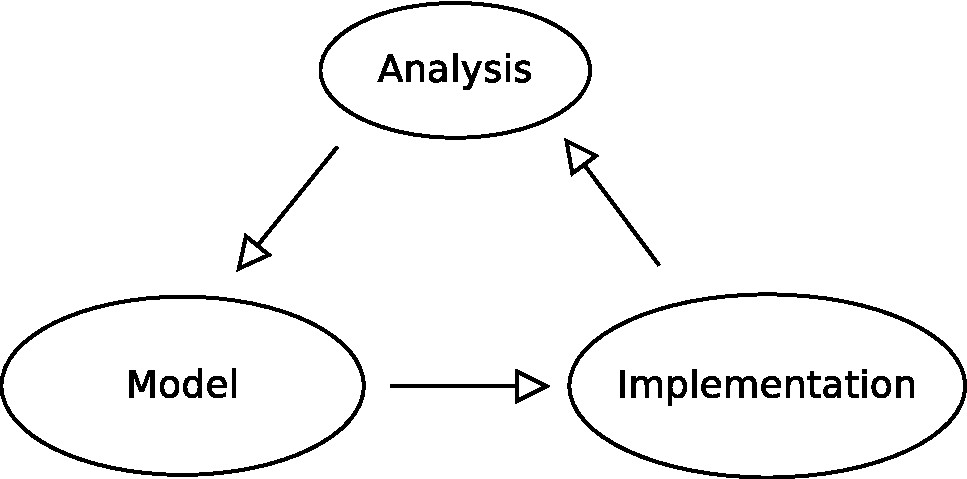
\includegraphics[height=6in]{methodology}}
        \else
        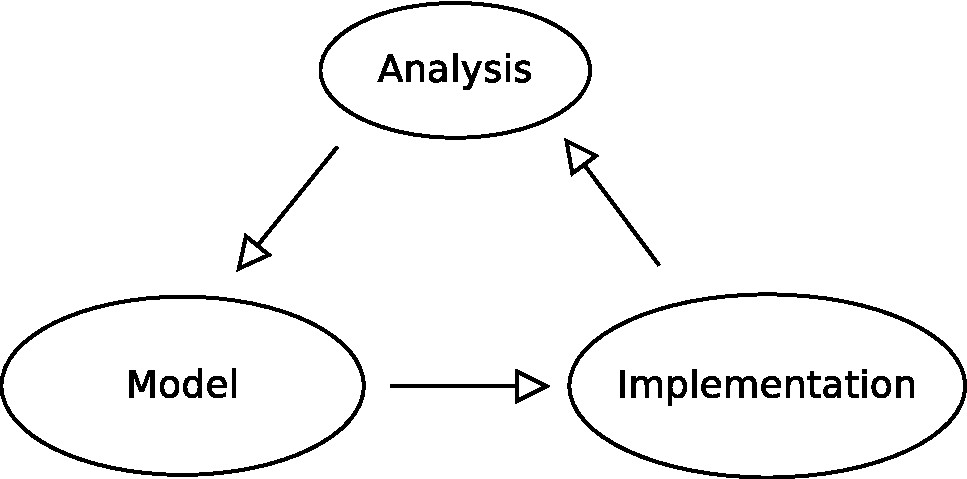
\includegraphics[bb = 92 86 545 742, height=6in]{methodology}
        \fi
        \caption{Instructional Simulate model for this study}
    \end{center}
\end{figure}

In the stage \verb|Model| and \verb|Implementation|, Use \verb|OPNET| as main tool. Because of \verb|OPNET| have provide a basic platform before progressing to the \verb|OBS| model. \verb|OPNET| simulation model library provide a series of simulation model for customer. On the basis of these simulation model, we can customize our network model and run a simulation. \verb|OPNET| simulation model library separate with the network simulation engine(\verb|OPNET|
Modeler,\verb|ITGuru|,Application DecisionGuru). This architecture is very convenient for model change and upgrade. For this study, we can deploy our congestion control algorithm to a \verb|OBS| network which build with \verb|OPNET| easily. 

To generate burst from all ingress node, we need to assume the arrive process follow certain distribution. That may be some common randomness processes. Such as negative exponential distribution, geometric distribution, drop-tail distribution. Thus we need to know how to generate this randomness process meet some distribution requirement. 

In order to measure our congestion control mechanism achievements. We need to setup a optimal target. In this study, that is maximum throughput and minimum burst loss and block ratio. It is hard to work out through pure analysis method. So we need to collect data from simulation. We can do some comparative experiments. Such as compare the throughput of two case. One with congestion control, the other without congestion control. Also, 
use some generally knowledge truth in queuing theory and probability theory to let us get closed optimal target step by step. It is a very good idea to make our data intuitive with data visualization technology.
